Pedestrian & Restricted Traffic Zones

A pedestrian zone is an urban area in which motorized vehicle access is disallowed. In some instances, all wheeled vehicles (including bicycles) are banned from the zone. Barriers are typically put in place to physically obstruct motorized vehicles from entering. These barriers typically come in the form of bollards (pictured below) and can be either permanent or removable, if access is required for certain motorized vehicles. Pedestrian zones can be created temporarily by closing off a normal street to motorized traffic by placing temporary barriers. Alternatively, permanent pedestrian zones can be designed without motorized traffic in mind. \figref{PZA}, \figref{PZC}, and \figref{PZD} illustrate examples of permanent pedestrian zones \cite{PZ4}.
 
\begin{figure}[h]
\centering
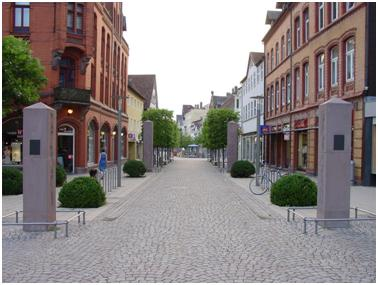
\includegraphics[width=\textwidth]{PZA.JPG}
\caption[Example of pedestrian zone design]{Example of pedestrian zone design: enough space allowed in the middle for essential motor vehicles, textured pavements to indicate an alternative purpose for the space, and bike racks in place to encourage bicycle use.}\label{fig:PZA}
\end{figure}

\begin{figure}[h]
\centering
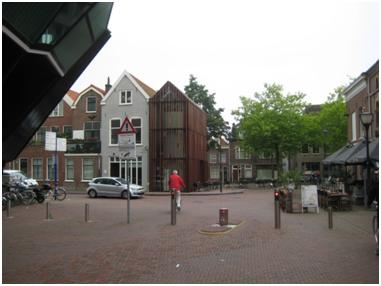
\includegraphics[width=\textwidth]{PZB.JPG}
\caption[Bollards restricting access to a pedestrian area]{Bollards restricting access to a pedestrian area}\label{fig:PZB}
\end{figure}

\begin{figure}[h]
\centering
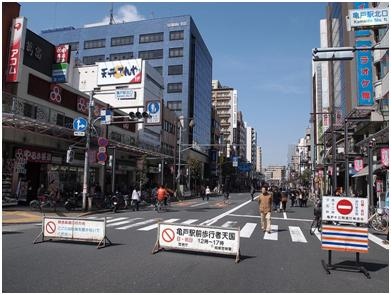
\includegraphics[width=\textwidth]{PZC.JPG}
\caption[A temporary pedestrian zone in Tokyo]{A temporary pedestrian zone in Tokyo, created by placing temporary barriers in front of a normal street}\label{fig:PZC}
\end{figure}

Pedestrians zones make land that was previously used for roads or parking available for gathering space or green space. Pedestrian zones increase the local populationís use of walking as a mode of transportation, which in turn decreases usage of automobiles, as businesses in the zone have increased their accessibility to pedestrians. Additionally, these zones are also known to increase rates of physical activity, particularly amongst children \cite{PZ4}.
 
\begin{figure}[h]
\centering
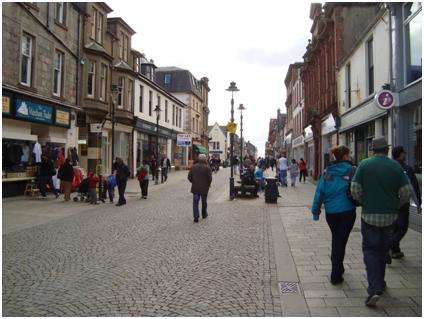
\includegraphics[width=\textwidth]{PZD.JPG}
\caption[A pedestrian zone]{A pedestrian zone}\label{fig:PZD}
\end{figure}

Restricted Traffic Zones are urban areas where non-essential motorized traffic is disallowed. This is a practice most commonly found in Italy, know as a \emph{zona traffico limatato}. The practice is used to reduce congestion and pollution in historical city centers. Cameras are placed at strategic checkpoints entering the zone to check control access. A picture is taken of every vehicle, and its license plate is cross-referenced against a list of permitted vehicles. Prohibited vehicles are fined. Depending on the characteristic of the restricted zone, other vehicles can be allowed as well, such as merchant vehicles, taxis, emergency vehicles, maintenance vehicles, and diplomats \cite{PZ1}. In combination with the closure of these zones to non-essential traffic, Italian cities increased public transit services to improve mobility. In Milan, for example, this practice proved to reduce automobile traffic in the zone by 50%. In Freiburg, Germany, traffic restriction and public transit improvements caused bicycle usage to double from 1976 to 1986 and led 18% of drivers to switch to public transit \cite{PZ2}. 
 
\begin{figure}[h]
\centering
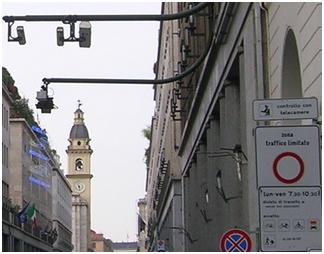
\includegraphics[width=\textwidth]{PZE.JPG}
\caption[\emph{Zona traffico limatato} warning sign and accompanying cameras]{\emph{Zona traffico limatato} warning sign and accompanying cameras}\label{fig:PZE}
\end{figure}

Costs

The primary costs of a restricted traffic zone are the construction and maintenance of the monitoring equipment; however, the fines (starting at an equivalent of $50 in Italy) collected due to violations would make up the difference \cite{PZ1}. One problem with these fines is that it is a nuisance to unsuspecting tourists who are not aware of the laws and fines. Additionally, if measures arenít taken to reduce total automobile traffic through public transit improvements, the traffic that is redirected due to these restrictions could cause significant congestion in other city zones.

The cost of introducing a pedestrian zone to an urban area depends on its design. Table A lists selected pedestrian improvements that could potentially be implemented in a pedestrian zone, and their estimated costs based on data from the San Francisco Bay Areaís Metropolitan Transportation Commission \cite{PZ8}.

[TABLE HERE NAKUL] Table A. Cost estimates of various elements of pedestrian zones \cite{PZ3}.
 
Total maintenance costs would also be dependent on the particular facilities. For an example of these costs, one can look to Corona Plaza in New York City. This proposed plaza is currently a dilapidated access road and parking lot, and is planned to be converted to a 13,000 square foot pedestrian public space \cite{PZ10}. It is estimated that it will cost between $50,000 and $75,000 a year to maintain this plaza \cite{PZ11}.
